\documentclass[a4paper,twocolumn]{article}

\usepackage[english]{babel}
\usepackage[utf8]{inputenc}
\usepackage{graphicx}
\usepackage{caption}
\usepackage{fullpage}

\newenvironment{Figure}
  {\par\medskip\noindent\minipage{\linewidth}}
  {\endminipage\par\medskip}

\title{Progressive Neural Networks $-$ summary}
\author{Matěj Nikl}

\begin{document}
\maketitle
Progressive Neural Networks (PNNs) are networks trying to address the task of using, transfering and not forgetting previously learned knowledge to learn yet another task, preferably with faster convergence. It retains a pool of trained models throughout training and learns connections to them to harvest potentially useful features while also learning new ones. What it means is that it has the ability to choose whether the previously learned knowledge is useful for the new task and thus transfer it, or on the other hand even ignore it completely (by zeroing the lateral connections).

    \begin{figure}[!h]
        \centering
        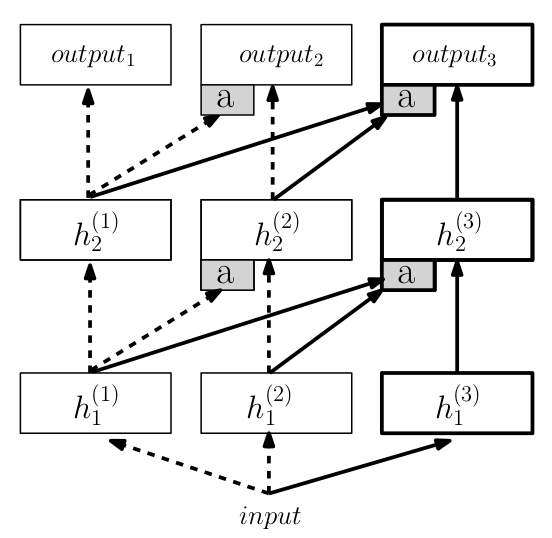
\includegraphics[width=0.8\columnwidth]{PNN.png}
        \captionof{figure}{A three column progressive network}
    \end{figure}

\subsection*{Principles of modularization}
The basic building block of PNNs is a \textit{column}. A column is a neural network with lateral connections to all previously trained columns, each trying to solve just one task. That might encourage the thinking of a column as a potential module. However, it cannot be taken away and used on its own as a some kind of standalone unit $-$ it always needs all of its previous columns with whom it was trained with to function properly, because it might be extremely dependent on features (knowledge) extracted from input by them. So, even though we might like to see it as a module, it definately cannot be used that way.


\subsection*{Principles of growing}
For each new task a new column is allocated. The knowledge from all previously learned tasks has the potencial to be transferred, while being protected against forgetting, because all previous columns have frozen weights.


    \begin{figure*}[ht]
        \centering
        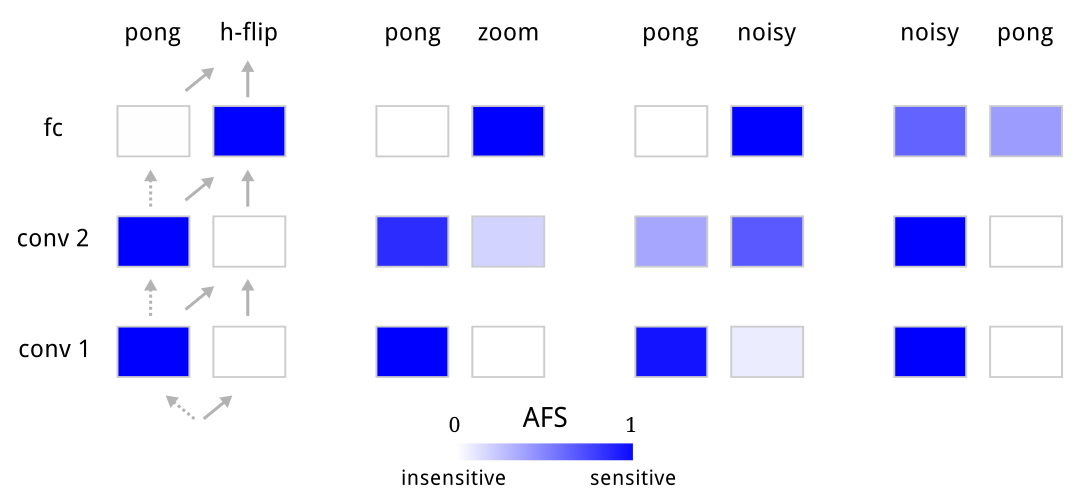
\includegraphics[width=0.9\textwidth]{2-column.png}
        \captionof{figure}{A two column progressive network $-$ knowledge transfer}
    \end{figure*}

    \begin{figure*}[ht]
        \centering
        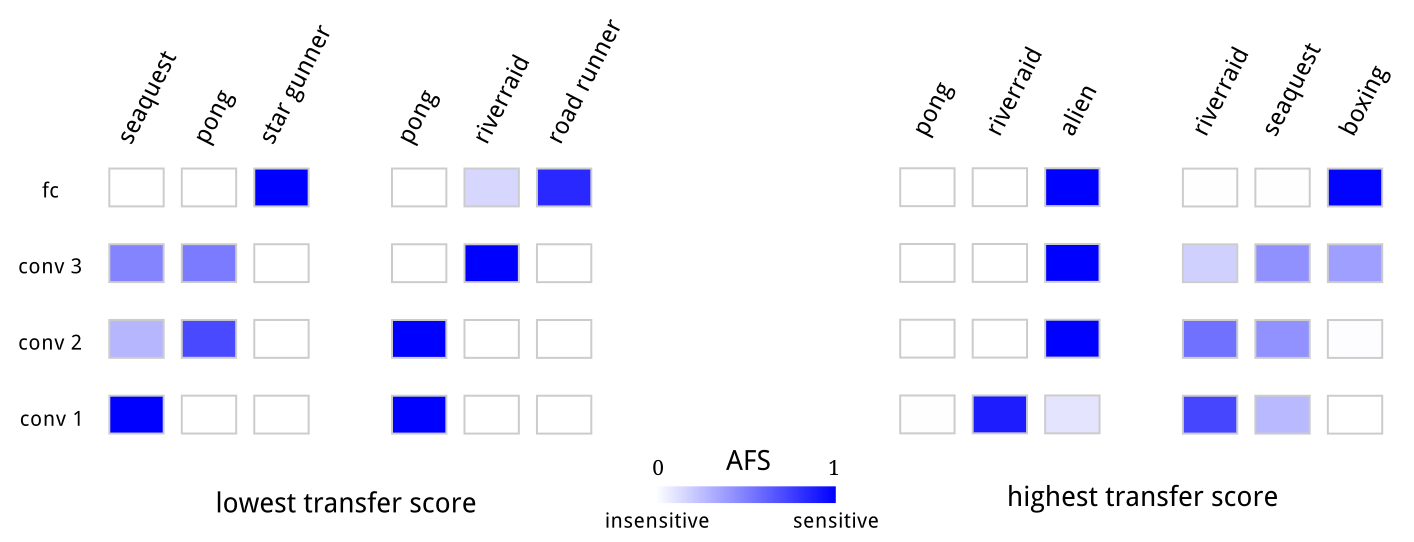
\includegraphics[width=0.9\textwidth]{3-column.png}
        \captionof{figure}{A three column progressive network $-$ knowledge transfer}
    \end{figure*}

    \begin{figure*}[ht]
        \centering
        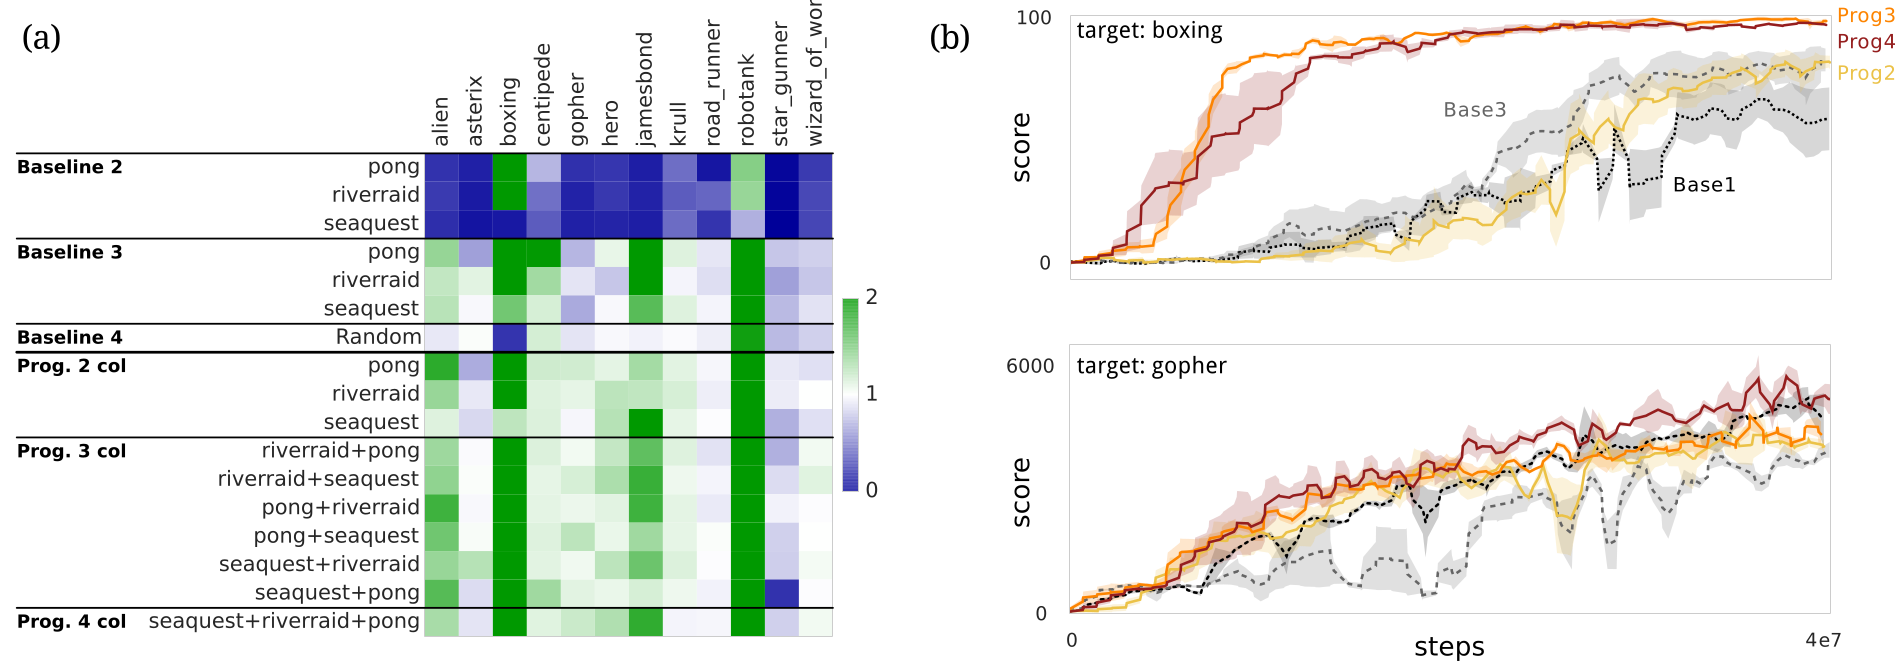
\includegraphics[width=\textwidth]{perf.png}
        \captionof{figure}{(a) Transfer matrix. Colours indicate transfer scores (clipped at 2). For progressive nets, the first column is trained on Pong, Noisy, or H-flip (table rows); the second column is trained on each of the other pong variants (table columns). (b) Example learning curves. Baseline 1 is a single column trained on the target task; baseline 2 is a single column, pretrained on a source task and finetuned on the target task (output layer only); baseline 3 is the same as baseline 2 but the whole model is finetuned; and baseline 4 is a 2 column progressive architecture, with previous column(s) initialized randomly and frozen.}
    \end{figure*}

\end{document}
